\section{Introduction}

\plainMHCI{} molecules display intracellularly derived peptides at the cell surface for surveillance by cytotoxic CD8-positive T cells (CD8\(^{+}\) T cells). The resulting immunopeptidome is shaped by substantially more than peptide binding to an \plainMHC{}: protein abundance and turnover, proteolytic degradation, antigen-processing pathways, cellular composition, tissue environment, and experimental detectability can all affect which peptides are observed. Multi-tissue immunopeptidomic studies have consequently revealed both widely shared ligands and pronounced tissue-associated differences \cite{marcu2021atlas,schuster2018mouse}. Nevertheless, most computational models are designed to predict peptide binding to or presentation by an \plainMHC{} in a general setting and therefore do not directly characterize how presentation evidence varies across tissues under a fixed antigen-presenting-molecule context (MHC context).

Tissue-associated presentation preference by \plainMHCI{} can arise at several successive stages of antigen processing. Genes encoding constitutive or immunoproteasomal subunits, transporters associated with antigen processing 1 and 2 (TAP1/2), endoplasmic-reticulum aminopeptidases 1 and 2 (ERAP1/2), and components of the peptide-loading machinery are not expressed uniformly across tissues. Together with tissue-dependent source-protein abundance and cell-type composition, these differences can alter which proteins are cleaved, which peptide fragments enter the endoplasmic reticulum, how precursor peptides are trimmed, and which sufficiently stable peptide--\plainMHCI{} complexes are ultimately displayed at the cell surface \cite{kubiniok2022constitutive}. Thus, the same source protein may generate different presented epitopes in different tissues, while the same epitope may differ across tissues in the amount or likelihood of surface presentation. Understanding this variation is important for cancer therapy: it can help prioritize epitopes that are efficiently presented by tumors but minimally presented by essential normal tissues, thereby improving target selection and reducing potential on-target, off-tumor toxicity. In the present study, these mechanisms provide a biological explanation for tissue-associated preference rather than a causal claim, because the model does not directly measure gene expression or the activity of individual processing steps.

\begin{figure}[tbp]
\centering
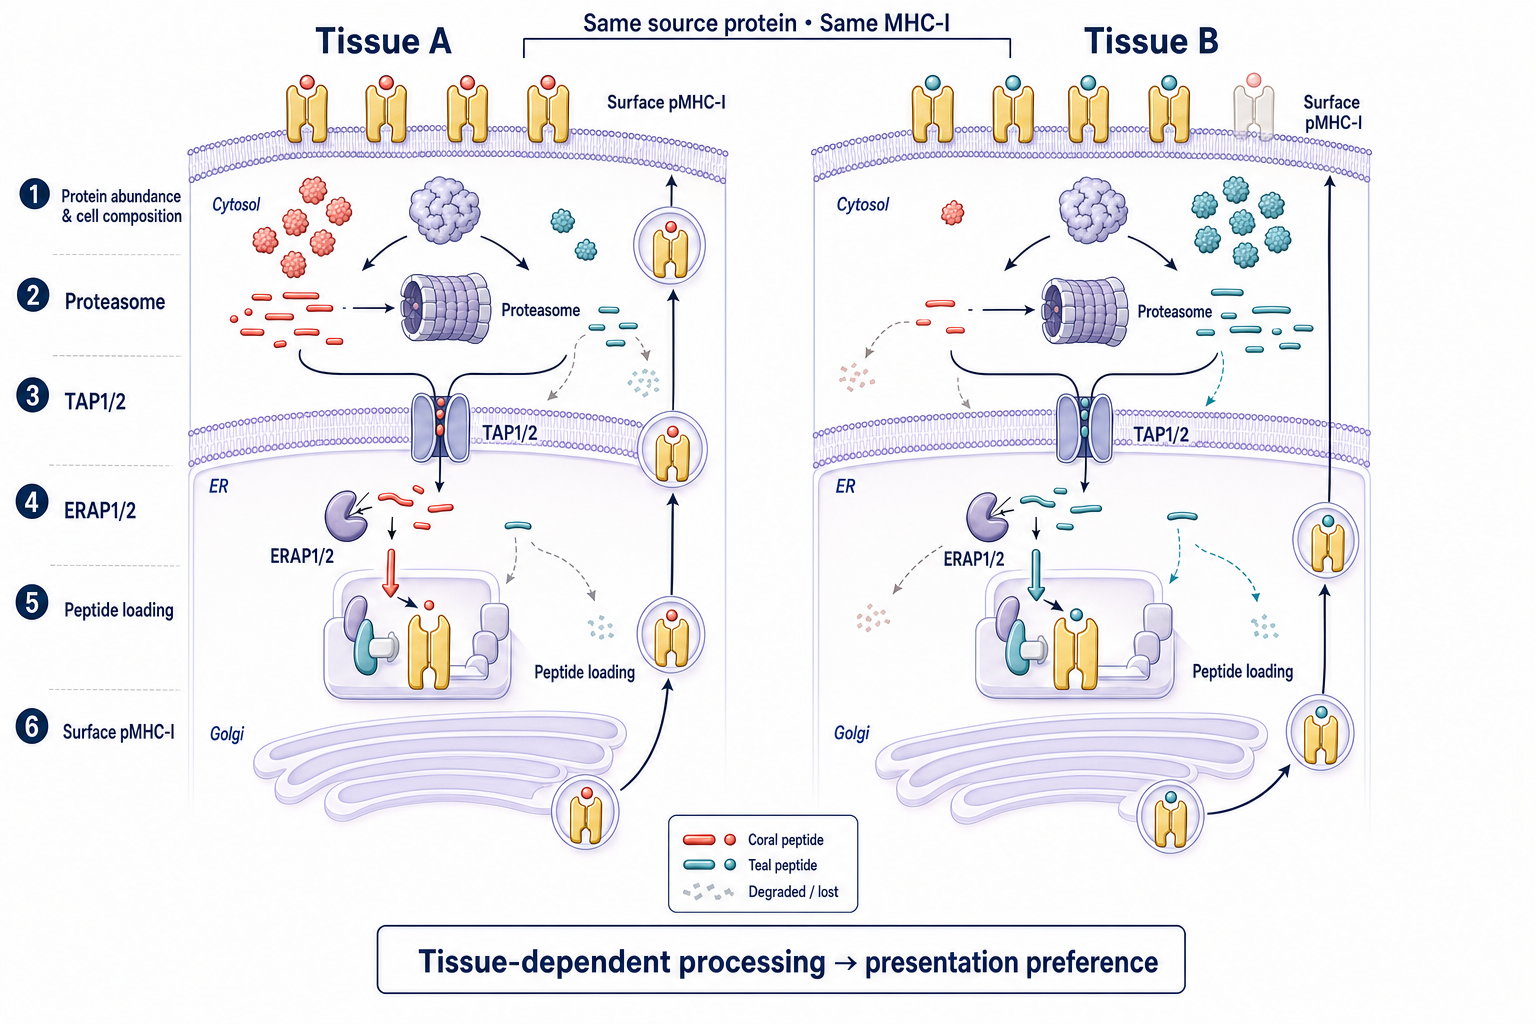
\includegraphics[width=\textwidth]{figures/tissue_specific_presentation_mechanism.png}
\caption{Conceptual mechanisms that can generate tissue-associated presentation preference by \plainMHCI{} under a fixed source-protein and antigen-presenting-molecule context (MHC context). Tissue-dependent source-protein abundance and cell-type composition, transport by proteins associated with antigen processing (TAP transport), trimming by endoplasmic-reticulum aminopeptidases (ERAP trimming), and peptide loading can enrich different peptides for surface display. Dashed paths denote peptide degradation or loss from the presented repertoire, not confirmed biological absence. The schematic motivates an association and does not establish causality for any individual processing step.}
\label{fig:tissue-specific-presentation-mechanism}
\end{figure}

Existing tools answer related but different questions. Some estimate whether a peptide can bind an \plainMHC{}; others estimate whether it is likely to be presented in a pooled or sample-specific setting, sometimes using expression or processing information \cite{reynisson2020netmhcpan,odonnell2020mhcflurry,albert2023bigmhc}. Here we ask a narrower relative question: when the antigen-presenting allele (MHC allele) and source protein are held constant, which of two peptides has stronger evidence in one specified tissue? Holding these two factors constant reduces easy explanations based only on compatibility with the antigen-presenting molecule (MHC compatibility) or protein identity and makes tissue-associated differences the focus of the comparison.

We call this question prediction of presentation preference for one tissue and one antigen-presenting restriction (\emph{tissue--MHC-specific presentation preference prediction}). Operationally, one prediction task corresponds to one tissue and one antigen-presenting restriction (MHC restriction). Let \(p\) denote a peptide and let \(\tau=(t,m)\) denote that tissue--antigen-presenting-molecule combination (tissue--MHC combination). A model produces a score
\[
s_{\theta}(p,\tau)\in\mathbb{R},
\]
which is used to rank peptides within that combination. A larger score means stronger predicted evidence relative to other candidates in the same task; it is not an absolute probability that the peptide is present. The model is evaluated only for tissue--antigen-presenting-molecule combinations (tissue--MHC combinations) represented during training, so it should not be interpreted as a predictor for a new tissue, a new antigen-presenting allele (MHC allele), or a new tissue--antigen-presenting-molecule combination (tissue--MHC combination).

To construct training examples aligned with this objective, each recorded-positive peptide is paired with a comparison peptide that has evidence elsewhere but not in the target tissue (a pseudo-negative peptide) under the constraints
\[
m^{+}=m^{-}, \qquad u^{+}=u^{-},
\]
where \(m\) is the antigen-presenting restriction (MHC restriction) and \(u\) is the parent UniProt protein. One peptide is reported in the target tissue; its comparison peptide sharing the presenting restriction and parent protein (matched comparison peptide) is reported elsewhere under the same \plainMHC{} and from the same protein, but not in the target task. Biologically, the pair asks whether two fragments of one protein show different tissue-associated evidence after controlling the presenting allele and source-protein identity. The second peptide is a comparison peptide with evidence elsewhere but not in the target tissue (\emph{pseudo-negative}), not a confirmed biological absence. Missing reports can reflect incomplete sampling or limited mass-spectrometry detection, and the pairing cannot remove study, batch, expression, or cell-composition effects.

On this basis, we introduce paired human and mouse TissuePMHC benchmarks and a human prediction model. The model combines a globally shared peptide representation with a representation restricted to one \plainHLA{} allele; in biological terms, this allows broadly shared sequence patterns and allele-associated motifs to contribute separately. The internal evaluation that keeps complete pairs out of training (standard evaluation) makes a test peptide absent from the current task's fitting rows but allows it to recur in another task. The \plainPeptideOOF{} additionally removes every held-out peptide from every fitting task. The latter tests tissue-associated ranking for unseen peptide identities within previously represented tissue--antigen-presenting-molecule combinations (tissue--MHC combinations).

The study makes four main contributions. First, it defines a biologically motivated comparison in which antigen-presenting restriction (MHC restriction) and parent protein are matched. Second, it provides human and mouse benchmarks built with the same minimum number of pairs required for a tissue--antigen-presenting-molecule combination to be retained (task-size requirement). Third, it measures how much performance falls when exact peptide identities cannot be reused across training and evaluation. Fourth, it tests whether the remaining signal depends on tissue identity or can be explained by general peptide--antigen-presenting-molecule compatibility (peptide--MHC compatibility) alone. The aim is therefore not only to report a high score, but also to clarify what biological question each score can and cannot answer.
